\section*{Questão 1 - HMM}

Considere o robô da lista anterior, que pode se mover pelos quadrados da figura abaixo.

\begin{figure}[H]
    \centering
    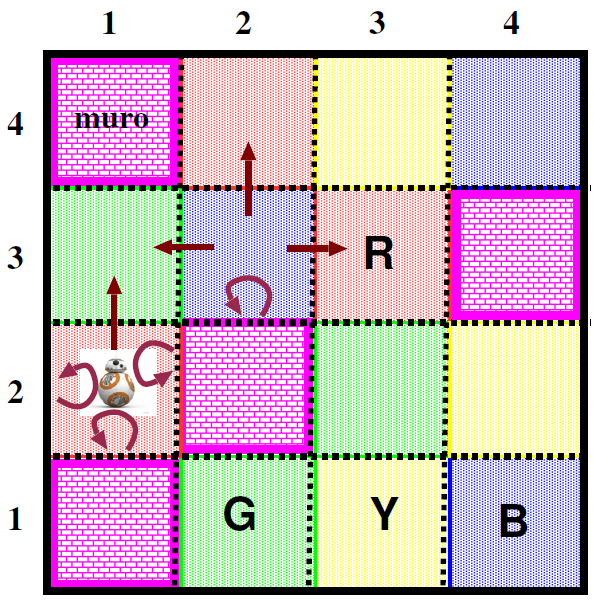
\includegraphics[width=0.5\textwidth]{fig/enunciado_q1.png}
    \caption{Robô andando por um ambiente}
    \label{fig:q1}
\end{figure}   

Para tentar melhorar a previsibilidade de se detectar a posição do robô da Figura \ref{fig:q1} sensores são colocados no ambiente onde o robô circula. Há 4 tipos de sensores (\textbf{R, B, Y, G}), conforme mostrado na Figura \ref{fig:q1}. Quando o robô está em qualquer um dos quadrados, o respectivo sensor emite um sinal (para um receptor) com a letra igual ao tipo do sensor. Entretanto, os sensores não são perfeitos e podem emitir um sinal errado com probabilidade 0.1. Por exemplo, quando o robô está num dos quadrados azuis, emite um sinal b com probabilidade 0.9, ou um dos restantes sinais r ou y ou g, com probabilidade 0.1/3. Como outro exemplo, suponha que o robô esteja na posição inicial conforme mostrado na Figura \ref{fig:q1}. Em 3 unidades de tempo, uma possível sequência de sinais recebidos poderiam ser \textbf{r g b}, se o robô for para norte e depois para leste. Entretanto, mesmo com o mesmo movimento, os sinais recebidos poderiam ser também \textbf{r g g} ou \textbf{b b b}, etc.

Seu objetivo é determinar a posição do robô, a partir dos sinais recebidos dos sensores.

\begin{itemize}
    \item \textbf{Explique como você fará uma HMM que possa permitir prever a posição do robô a partir dos sinais recebidos.}
    \begin{tcolorbox}[title=Resposta:]

    \begin{enumerate}
        \item \textbf{Estados:} Assim como no problema da lista anterior, os estados são as posições possíveis do robô, com a diferença de que agora os estados não podem ser diretamente observáveis. Para facilitar a notação, os estados foram numerados em ordem crescente da esquerda para a direita e de cima para baixo. Assim, o antigo estado (1,1) passou a se chamar $S_1$, (1,2) passou a se chamar $S_2$ e assim por diante. O modelo da Cadeia de Markov pode sewr visto na figura \ref{fig:cadeia_markov}.
        \item \textbf{Observações:} As observações são as emissões dos sensores, formadas pelos símbolos \textbf{R, B, Y, G}. 
        \item \textbf{Matriz de transição:} A matriz de transição é a mesma da lista anterior, com as probabilidades de transição entre os estados. Nesta lista foi utilizada a letra $A$ para representar a matriz de transição, seguindo a simbologia de Rabiner (1989) \cite{Rabiner1989}. A matriz $A$ é mostrada na tabela \ref{tab:matriz_transicao_a}.
        \item \textbf{Matriz de emissão:} A matriz de emissão é a probabilidade de cada estado emitir cada uma das observações. Cada estado tem uma probabilidade de 0.9 de emitir a cor dele mesmo e 0.1 de emitir qualquer outra cor ($0.1/3 \approx 0.0333 $ para cada cor). Os estados proibidos (rosa) possuem probabilidade de emissão 0 para todos os símbolos. A matriz de emissão é mostrada na tabela \ref{tab:matriz_emissao_b}.
        \item \textbf{Probabilidade inicial:} O vetor de probabilidades iniciais (renomeado para $\pi$ pelo mesmo motivo da matriz de transição) é o mesmo da lista anterior, com a probabilidade 1 do robô começar no estado $S_5$ (posição 2,1) $\pi_5=1$ e nula para os demais estados.
    \end{enumerate}

    \end{tcolorbox}

    \begin{figure}[H]
        \centering
        \begin{tikzpicture}[->, >=stealth, node distance=2cm, auto]
        
        % Define nodes with inverted y-axis and two-digit labels
        \node[state] (11) at (0,0) {$S_1$};
        \node[state] (12) [right=of 11] {$S_2$};
        \node[state] (13) [right=of 12] {$S_3$};
        \node[state] (14) [right=of 13] {$S_4$};
            
        \node[state] (21) [above=of 11] {$S_5$};
        \node[state] (22) [above=of 12] {$S_6$};
        \node[state] (23) [above=of 13] {$S_7$};
        \node[state] (24) [above=of 14] {$S_8$};
            
        \node[state] (31) [above=of 21] {$S_9$};
        \node[state] (32) [above=of 22] {$S_{10}$};
        \node[state] (33) [above=of 23] {$S_{11}$};
        \node[state] (34) [above=of 24] {$S_{12}$};
            
        \node[state] (41) [above=of 31] {$S_{13}$};
        \node[state] (42) [above=of 32] {$S_{14}$};
        \node[state] (43) [above=of 33] {$S_{15}$};
        \node[state] (44) [above=of 34] {$S_{16}$};


        % Transitions for node (1,2)
        \path (12) edge [loop below] node {0.75} (12) % Combined loop for south, west, and north (bottom border, wall at (1,1), wall at (2,2))
        edge[bend left] node[above] {0.25} (13);

        % Transitions for node (1,3)
        \path (13) edge [loop below] node {0.25} (13) % Loop for south (bottom border)
        edge[bend left] node[below] {0.25} (12)
        edge[bend left] node[above] {0.25} (14)
        edge[bend left] node[above] {0.25} (23);

        % Transitions for node (1,4)
        \path (14) edge [loop right] node {0.50} (14) % Combined loop for east and south (right border, bottom border)
        edge[bend left] node[below] {0.25} (13)
        edge[bend left] node[right] {0.25} (24);

        % Transitions for node (2,1)
        \path (21) edge [loop right] node {0.75} (21) % Combined loop for west, south, and east (left border, wall at (1,1), wall at (1,2))
        edge[bend left] node[above] {0.25} (31);

        % Transitions for node (2,3)
        \path (23) edge[bend left] node[below] {0.25} (13)
        edge [loop left] node {0.25} (23) % Loop for west (wall at (2,2))
        edge[bend left] node[above] {0.25} (24)
        edge[bend left] node[right] {0.25} (33);

        % Transitions for node (2,4)
        \path (24) edge [loop right] node {0.50} (24) % Combined loop for east and north (right border, wall at (3,4))
        edge[bend left] node[below] {0.25} (14)
        edge[bend left] node[below] {0.25} (23);

        % Transitions for node (3,1)
        \path (31) edge [loop left] node {0.50} (31) % Combined loop for west and north (left border, wall at (4,1))
        edge[bend left] node[below] {0.25} (21)
        edge[bend left] node[above] {0.25} (32);

        % Transitions for node (3,2)
        \path (32) edge[loop below] node {0.25} (32) % Loop for south (wall at (2,2))
        edge[bend left] node[below] {0.25} (31)
        edge[bend left] node[above] {0.25} (33)
        edge[bend left] node[right] {0.25} (42);

        % Transitions for node (3,3)
        \path (33) edge[bend left] node[below] {0.25} (23)
        edge[bend left] node[below] {0.25} (32)
        edge[loop right] node {0.25} (33) % Loop for east (wall at (3,4))
        edge[bend left] node[right] {0.25} (43);

        % Transitions for node (4,2)
        \path (42) edge [loop above] node {0.50} (42) % Combined loop for north and west (top border, wall at (4,1))
        edge[bend left] node[below] {0.25} (32)
        edge[bend left] node[above] {0.25} (43);

        % Transitions for node (4,3)
        \path (43) edge [loop above] node {0.25} (43) % Loop for north (top border)
        edge[bend left] node[below] {0.25} (33)
        edge[bend left] node[below] {0.25} (42)
        edge[bend left] node[above] {0.25} (44);

        % Transitions for node (4,4)
        \path (44) edge [loop right] node {0.75} (44) % Combined loop for east, north, and south (right border, top border, wall at (3,4))
        edge[bend left] node[below] {0.25} (43);
        
        \end{tikzpicture}
        \caption{Cadeia de Markov representando o movimento do robô no ambiente.}
        \label{fig:cadeia_markov}
        \end{figure}


        \begin{table}[H]
            \centering
            \resizebox{0.9\textwidth}{!}{
                \begin{tabular}{c|cccccccccccccccc}
                      & $S_1$ & $S_2$ & $S_3$ & $S_4$ & $S_5$ & $S_6$ & $S_7$ & $S_8$ & $S_9$ & $S_{10}$ & $S_{11}$ & $S_{12}$ & $S_{13}$ & $S_{14}$ & $S_{15}$ & $S_{16}$ \\
                    \hline
                    $S_1$ & 0    & 0    & 0    & 0    & 0    & 0    & 0    & 0    & 0    & 0    & 0    & 0    & 0    & 0    & 0    & 0 \\
                    $S_2$ & 0    & 0.75 & 0.25 & 0    & 0    & 0    & 0    & 0    & 0    & 0    & 0    & 0    & 0    & 0    & 0    & 0 \\
                    $S_3$ & 0    & 0.25 & 0.25 & 0.25 & 0    & 0    & 0.25 & 0    & 0    & 0    & 0    & 0    & 0    & 0    & 0    & 0 \\
                    $S_4$ & 0    & 0    & 0.25 & 0.50 & 0    & 0    & 0    & 0.25 & 0    & 0    & 0    & 0    & 0    & 0    & 0    & 0 \\
                    $S_5$ & 0    & 0    & 0    & 0    & 0.75 & 0    & 0    & 0    & 0.25 & 0    & 0    & 0    & 0    & 0    & 0    & 0 \\
                    $S_6$ & 0    & 0    & 0    & 0    & 0    & 0    & 0    & 0    & 0    & 0    & 0    & 0    & 0    & 0    & 0    & 0 \\
                    $S_7$ & 0    & 0    & 0.25 & 0    & 0    & 0    & 0.25 & 0.25 & 0    & 0    & 0.25 & 0    & 0    & 0    & 0    & 0 \\
                    $S_8$ & 0    & 0    & 0    & 0.25 & 0    & 0    & 0.25 & 0.50 & 0    & 0    & 0    & 0    & 0    & 0    & 0    & 0 \\
                    $S_9$ & 0    & 0    & 0    & 0    & 0.25 & 0    & 0    & 0    & 0.50 & 0.25 & 0    & 0    & 0    & 0    & 0    & 0 \\
                    $S_{10}$ & 0    & 0    & 0    & 0    & 0    & 0    & 0    & 0    & 0.25 & 0.25 & 0.25 & 0    & 0    & 0.25 & 0    & 0 \\
                    $S_{11}$ & 0    & 0    & 0    & 0    & 0    & 0    & 0.25 & 0    & 0    & 0.25 & 0.25 & 0    & 0    & 0    & 0.25 & 0 \\
                    $S_{12}$ & 0    & 0    & 0    & 0    & 0    & 0    & 0    & 0    & 0    & 0    & 0    & 0    & 0    & 0    & 0    & 0 \\
                    $S_{13}$ & 0    & 0    & 0    & 0    & 0    & 0    & 0    & 0    & 0    & 0    & 0    & 0    & 0    & 0    & 0    & 0 \\
                    $S_{14}$ & 0    & 0    & 0    & 0    & 0    & 0    & 0    & 0    & 0    & 0.25 & 0    & 0    & 0    & 0.50 & 0.25 & 0 \\
                    $S_{15}$ & 0    & 0    & 0    & 0    & 0    & 0    & 0    & 0    & 0    & 0    & 0.25 & 0    & 0    & 0.25 & 0.25 & 0.25 \\
                    $S_{16}$ & 0    & 0    & 0    & 0    & 0    & 0    & 0    & 0    & 0    & 0    & 0    & 0    & 0    & 0    & 0.25 & 0.75 \\
                \end{tabular}
            }
            \caption{Matriz de Transição A}
            \label{tab:matriz_transicao_a}
        \end{table}

        \begin{table}[H]
            \centering
            \resizebox{0.9\textwidth}{!}{
                \begin{tabular}{c|cccccccccccccccc}
                      & $S_1$ & $S_2$ & $S_3$ & $S_4$ & $S_5$ & $S_6$ & $S_7$ & $S_8$ & $S_9$ & $S_{10}$ & $S_{11}$ & $S_{12}$ & $S_{13}$ & $S_{14}$ & $S_{15}$ & $S_{16}$ \\
                    \hline
                    R (Vermelho) & 0     & 0.0333  & 0.0333  & 0.0333  & 0.9000  & 0       & 0.0333  & 0.0333  & 0.0333  & 0.0333  & 0.9000  & 0       & 0      & 0.9000  & 0.0333  & 0.0333 \\
                    B (Azul)     & 0     & 0.0333  & 0.0333  & 0.9000  & 0.0333  & 0       & 0.0333  & 0.0333  & 0.0333  & 0.9000  & 0.0333  & 0       & 0      & 0.0333  & 0.0333  & 0.9000 \\
                    Y (Amarelo)  & 0     & 0.0333  & 0.9000  & 0.0333  & 0.0333  & 0       & 0.0333  & 0.9000  & 0.0333  & 0.0333  & 0.0333  & 0       & 0      & 0.0333  & 0.9000  & 0.0333 \\
                    G (Verde)    & 0     & 0.9000  & 0.0333  & 0.0333  & 0.0333  & 0       & 0.9000  & 0.0333  & 0.9000  & 0.0333  & 0.0333  & 0       & 0      & 0.0333  & 0.0333  & 0.0333 \\
                \end{tabular}
            }
            \caption{Matriz de Emissão \( B \)}
            \label{tab:matriz_emissao_b}
        \end{table}
    
    \item \textbf{Suponha que o receptor de sinais tenha recebido a sequência}
    r r y r y r b g b r y y g b. Qual a probabilidade desta sequência ocorrer? Explique e implemente o algoritmo necessário para responder a pergunta.
    \item \textbf{Repita o item anterior para a sequência}
    r b y r g r b g b r y y g b. (Obviamente não precisa reimplementar o algoritmo!)
    \item \textbf{Para a primeira sequência acima, qual o quadrado mais provável onde estará o robô na última posição (isto é, o quadrado de onde foi emitido o último sinal)? Explique e implemente o algoritmo necessário.}
    \item \textbf{Para a segunda sequência acima, qual o quadrado mais provável onde estará o robô?}
    \item \textbf{Para a primeira sequência acima, qual o caminho mais provável percorrido pelo robô? Explique o algoritmo usado, mas não precisa implementar. Use uma biblioteca de Python ou outra linguagem preferida.}
\end{itemize}

% Espaço para figura da questão 1

